\documentclass[fontset=none]{ctexart}

\usepackage[T1]{fontenc}
\usepackage{fontspec}
\setCJKmainfont{SimSun}
% Latin Modern
\renewcommand*\ttdefault{txtt} % 改等宽字体

\setcounter{tocdepth}{5}
\setcounter{secnumdepth}{5}
% -1 part
% 0 chapter
% 1 section
% 2 subsection
% 3 subsubsection
% 4 paragraph
% 5 subparagraph

\usepackage{cite}
\usepackage{geometry}
\geometry{a4paper,scale=0.7}

\usepackage{algorithm}  
\usepackage{algorithmicx}  
\usepackage{algpseudocode}
\makeatletter
\newenvironment{breakablealgorithm}
  {% \begin{breakablealgorithm}
   \begin{center}
     \refstepcounter{algorithm}% New algorithm
     \hrule height.8pt depth0pt \kern2pt% \@fs@pre for \@fs@ruled
     \renewcommand{\caption}[2][\relax]{% Make a new \caption
       {\raggedright\textbf{\ALG@name~\thealgorithm} ##2\par}%
       \ifx\relax##1\relax % #1 is \relax
         \addcontentsline{loa}{algorithm}{\protect\numberline{\thealgorithm}##2}%
       \else % #1 is not \relax
         \addcontentsline{loa}{algorithm}{\protect\numberline{\thealgorithm}##1}%
       \fi
       \kern2pt\hrule\kern2pt
     }
  }{% \end{breakablealgorithm}
     \kern2pt\hrule\relax% \@fs@post for \@fs@ruled
   \end{center}
  }
\makeatother

\usepackage{amsmath}
\usepackage{amssymb}
\usepackage{graphicx}
\usepackage{subfigure}
\usepackage{changepage}
\usepackage{multirow}
\usepackage{url}

\usepackage{amsthm}
\newtheorem{theorem}{Theorem}[section]
\newtheorem{lemma}[theorem]{Lemma}
\newtheorem{proposition}[theorem]{Proposition}
\newtheorem{corollary}[theorem]{Corollary}
% \newtheorem{remark}{Remark}[section]
\newtheorem{example}{Example}[section]
\newenvironment{solution}{\begin{proof}[Solution]}{\end{proof}}
\theoremstyle{definition}
\newtheorem{definition}{Definition}[section]
\theoremstyle{remark}
\newtheorem*{remark}{Remark}

\usepackage[colorlinks, linkcolor=black, citecolor=blue, bookmarksnumbered]{hyperref}
% \hypersetup{
% 	colorlinks=true,
% 	linkcolor=cyan,
% 	filecolor=blue,      
% 	urlcolor=red,
% 	citecolor=green,
% }

\usepackage{fancyhdr}
\pagestyle{fancy}
\renewcommand{\sectionmark}[1]{\markright{\thesection\ #1}}
\fancyhf{}
\cfoot{\thepage}
\lhead{\rightmark}
% \rightmark 当前的节名
% \leftmark 当前的章名
% \(l/c/r)head{}, \(l/c/r)foot{}
\renewcommand{\headrulewidth}{0.4pt}
\renewcommand{\footrulewidth}{0pt}

\renewcommand\refname{References}
\renewcommand\contentsname{Content}
\renewcommand\figurename{Figure}

\begin{document}

\begin{titlepage}
    \begin{center}
        \vspace*{1cm}
            
        \Huge
        \textbf{Design and Implementation of A TTE System}
            
        \vspace{0.5cm}
        \LARGE
        Second Report\\
            
        \vspace{1.5cm}
            
        \textbf{11812804}  董\quad 正\\
        \textbf{11813225}  王宇辰\\
        \textbf{11811305}  崔俞崧\\

        \vspace{0.5cm}
        Supervisior: 宋轩
            
        \vfill
            
        
\includegraphics[width=\textwidth]{images/sustc.png}
            
        \vspace{0.2cm}
            
        \Large
        Department of Computer Science and Engineering\\
        \vspace{0.5cm}
        May. 2021
            
    \end{center}
\end{titlepage}

\tableofcontents

\clearpage
\section{Preliminaries}
\subsection{Review}
\subsubsection{TTE}
\textbf{Travel Time Estimation (TTE)} is one of the most important researching topic in the traffic forecasting field. 
Estimating the travel time of any path in a city is of great importance to traffic monitoring, route planning, ridesharing, taxi dispatching, etc.
On Sep. 2020, DeepMind published a blog named \textit{Traffic prediction with advanced Graph Neural Networks}. 
This blog briefly described the whole industrial structure of estimated times of arrival (ETAs) techniques applied in Google Map but did not given any detailed implementation or any code.
Our work is based on the model structure of TTE proposed in the blog.
\begin{figure}[htb]
    \centering
    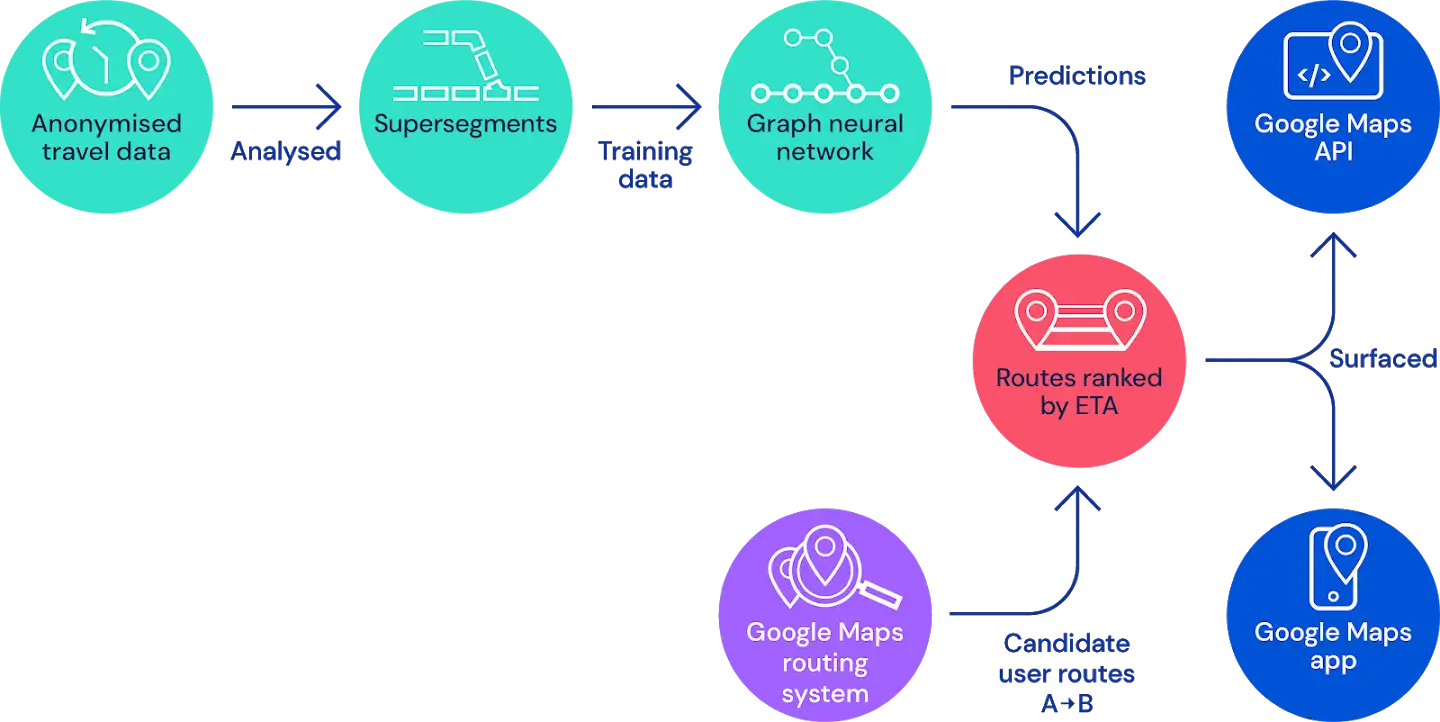
\includegraphics[width=0.9\textwidth]{images/architecture.png}
    \caption{Architecture}
    \label{fig1}
\end{figure}

\subsubsection{Goal}
Our ultimate goal (tentative) is to implement the industrial structure and apply it to the open source databases in China, then compare the performance with the state-of-the-art structures and find its application value.
This semester, we will implement a TTE system base on the work we done in the last term, combining \textit{Supersegment} and TTI.
We will try to work out an interactive application with graphical user interface. 

\subsection{Introduction}
In last stage, we finished the code of \textit{Supersegment} and made a simple UI design of our application.

Breifly, we will state our work in this report as
\begin{itemize}
  \item TTE Web APP Design by 董正 \& 王宇辰
  \item Result Analysis on \textit{TTI} and \textit{Supersegment} by 崔俞崧
\end{itemize}

\section{TTE Web APP Design}
\subsection{Introduction}
Our application is a front-back web system.

Front end:
\begin{itemize}
  \item \textit{Leaflet}: A JavaScript map library
  \item \textit{高德地图}: Provider of the base map
  \item \textit{jQuery}: A JavaScript communicator
\end{itemize}

Back end:
\begin{itemize}
  \item \textit{Flask}: A \textit{Python} back-end framework
  \item \textit{NetworkX}: A \textit{Python} library for graph analysis
  \item \textit{GeoJSON}: A special format of JSON that represents geo data
\end{itemize}

\subsection{Implementation}
\begin{enumerate}
  \item Convert orginal road data to \textit{shapefile} format
  \item Build geo-graph with \textit{NetworkX}
  \item Select start and end points in web front, use \textit{jQuery} to send request to back-end server
  \item Run \textit{Dijkstra} alogrithm in the graph to find shortest path and distance
  \item Send \textit{GeoJSON} data to front-end and show the calculated path
  \item Calculate TTI, and use it to work out the estimated time of arrival
  \item Send the final result to front-end
\end{enumerate}

\begin{figure}[htb]
  \centering
  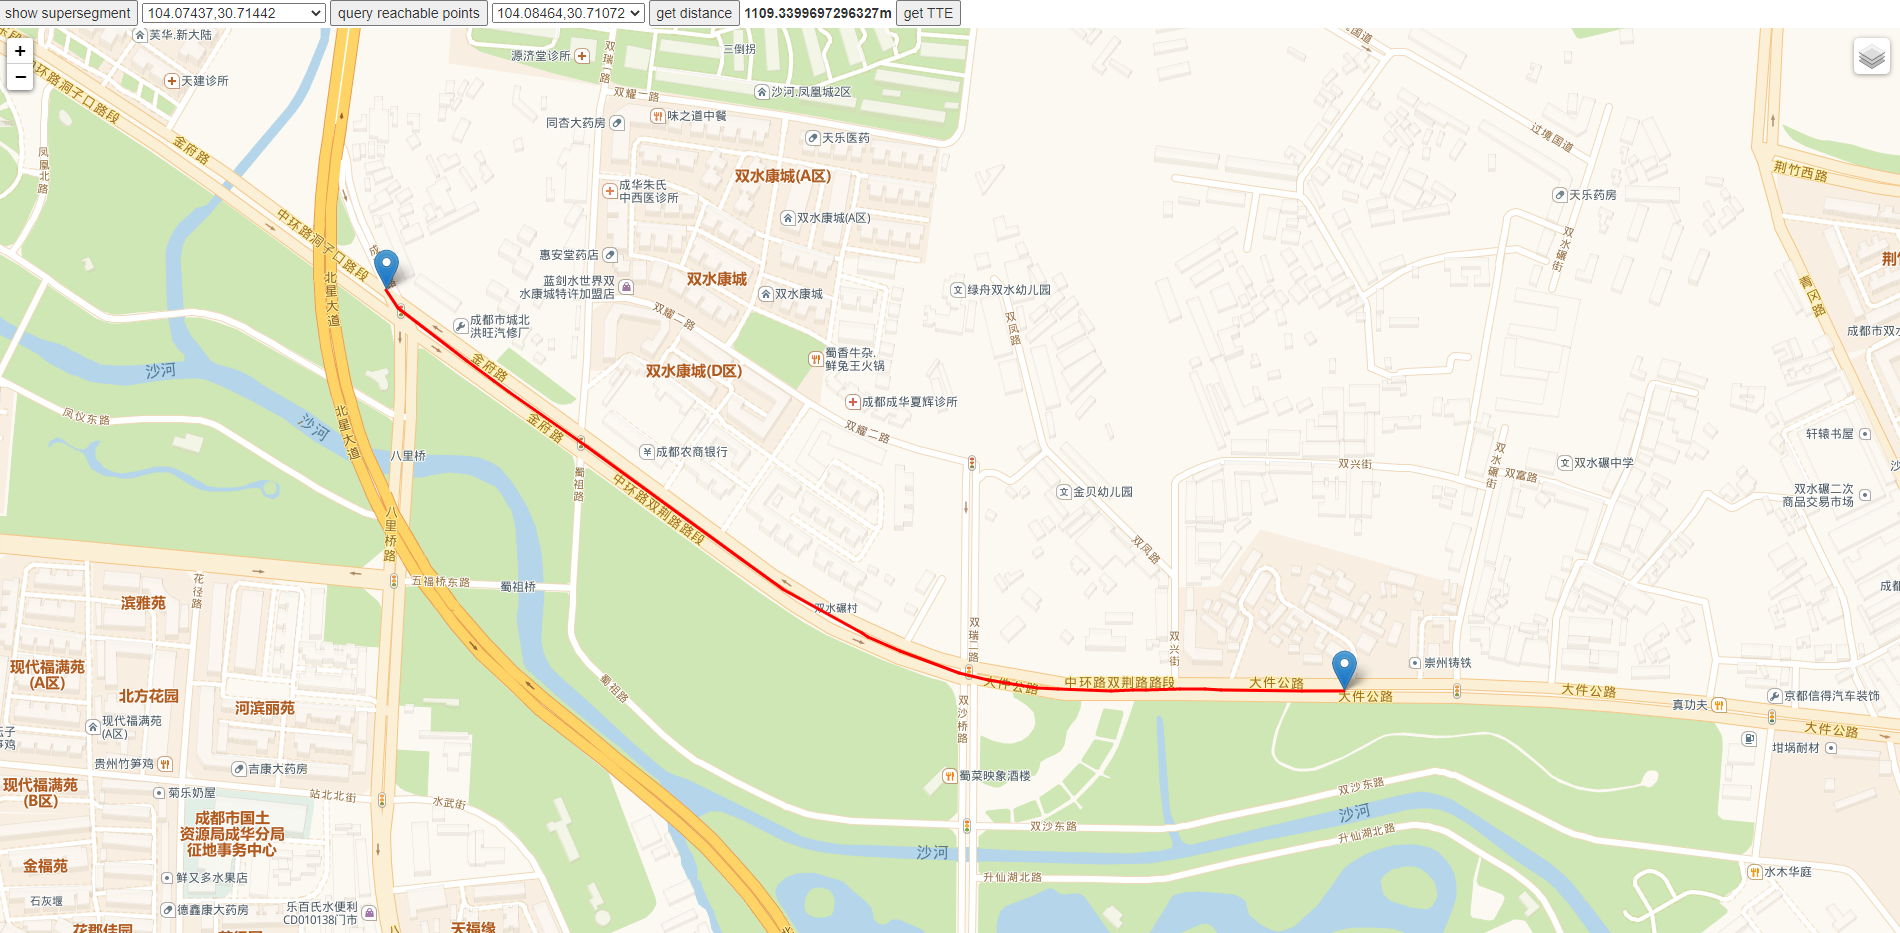
\includegraphics[width=\textwidth]{images/app_example.png}
  \caption{Web Application}
  \label{app}
\end{figure}

\section{Result Analysis on TTI and Supersegment}
\subsection{Purpose of Result Analysis}
The main purpose of error analysis is to analyze the current results, compare them with the actual values, find out the shortcomings of the current algorithm and improve these algorithms. First of all, the two algorithms are still relatively rough, while the current evaluation methods are still not clear. By calculating the error of travel time prediction, we can find out whether the accuracy can be improved after improving the algorithms. Secondly, by comparing the two algorithms with the average speed of difference roads, we can know whether the two algorithms could improve the time prediction, and whether they could be a means of data preprocessing for neural network.

\clearpage
\subsection{Results of Current Error Analysis}
\begin{figure}[htb]
  \centering
  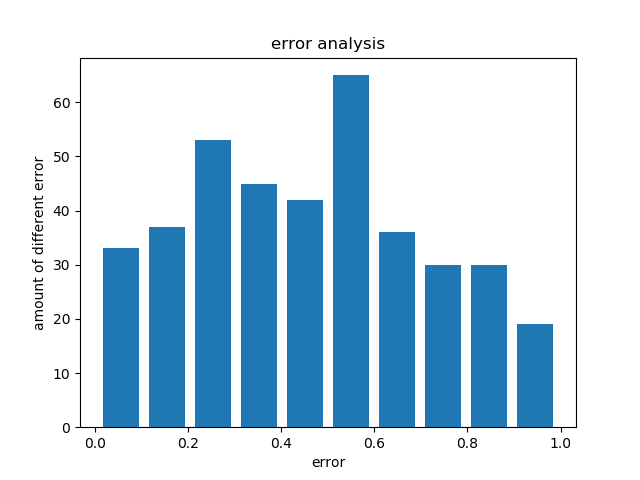
\includegraphics[width=\textwidth]{images/error1.png}
  \caption{Prediction using road's average speed}
  \label{error1}
\end{figure}

\begin{figure}[htb]
  \centering
  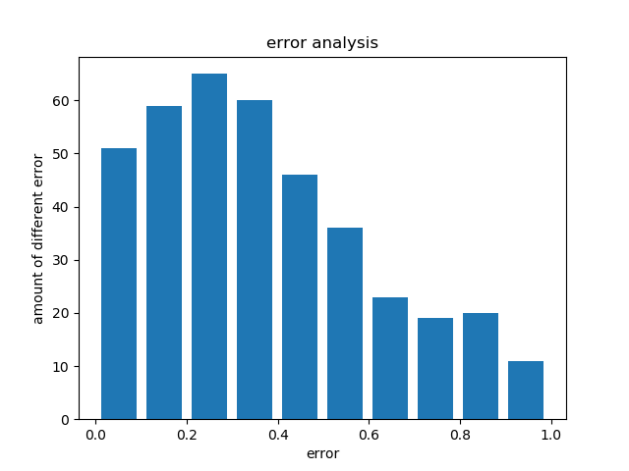
\includegraphics[width=\textwidth]{images/error2.png}
  \caption{Prediction using road's TTI}
  \label{error2}
\end{figure}

\begin{figure}[htb]
  \centering
  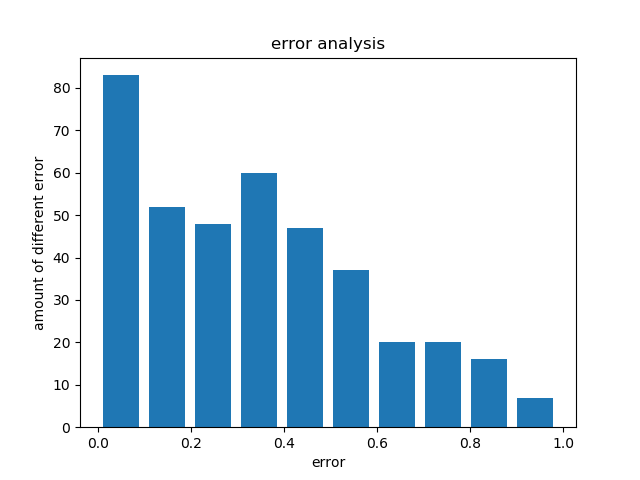
\includegraphics[width=\textwidth]{images/error3.png}
  \caption{Prediction using Supersegment}
  \label{error3}
\end{figure}

\clearpage
\subsection{Interpretation of Results}
As can be seen from the results of 3.2, both algorithms improves the accuracy of time prediction. The improvement of TTI is more pronounced than SuperSegment. Analytical reasons is that the current forecast is based on the road rather than the trajectory. And vehicles are more likely travel the entire road, in which case using supersegment or not will not make a big difference in results. However, TTI is closely related to travel time, and there are obvious differences in TTI at different time.

It can also be seen from the results that there are still errors in the prediction results, which are related to the processing process of the algorithm and the particularity of the trajectory

In addition, the amount of data used in the current calculation is still too small, which also has some reasons for the error. Too little data can lead to too many generalizations, making it harder to deal with extreme cases. More data will improve the accuracy of the results.

Finally, in order to ensure the efficiency of the algorithm, there will be some errors in the calculation process, and these errors will eventually be reflected in the error of time prediction.

\subsection{Ascending Direction}
\begin{enumerate}
  \item Increase the amount of data and improve the efficiency of the algorithm, so that more data can be used to build the model and the algorithm can better deal with special cases.
  \item Improve TTI and Supersegment algorithms to increase the accuracy of the models. At present, the algorithms still has some approximate cases, in addition, the treatment of special cases is not perfect. How to improve the algorithm and make the model more accurate is one way to improve the prediction accuracy.
  \item TTI and Supersegment could be considered as parameter preprocessing means for time series analysis and neural network. At present, parameter input of Deep learning models such as DeepTTE is only simple road section and trajectory data. If it is pretreated to a certain extent, the accuracy of prediction may be improved.
\end{enumerate}

% \clearpage
% \phantomsection
% \addcontentsline{toc}{section}{References}
% \bibliographystyle{ieeetr}
% \bibliography{references}

\end{document}